\documentclass[tikz,border=10pt]{standalone}
\begin{document}
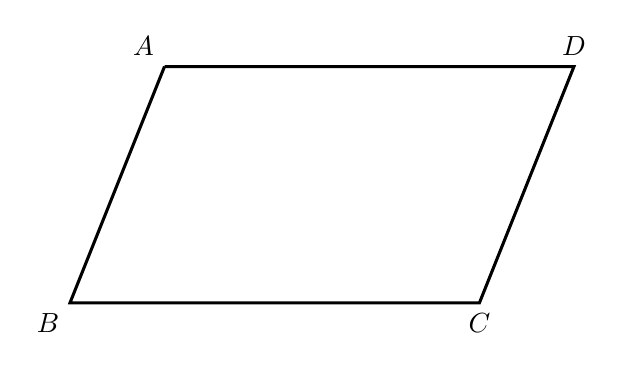
\begin{tikzpicture}[line width=1.1pt]
  \coordinate (A) at (1.8,3.2);
  \coordinate (B) at (0.6,0.2);
  \coordinate (C) at (5.8,0.2);
  \coordinate (D) at (7.0,3.2);

  \draw (A) -- (B) -- (C) -- (D) -- (A);

  \node[above left] at (A) {$A$};
  \node[below left] at (B) {$B$};
  \node[below] at (C) {$C$};
  \node[above] at (D) {$D$};
\end{tikzpicture}
\end{document}
